% Chapter 1
\chapter{Marco Teórico} % Main chapter title

\label{Cap_Marco} % For referencing the chapter elsewhere, use \ref{Cap_Marco} 

%----------------------------------------------------------------------------------------

% Define some commands to keep the formatting separated from the content 
\newcommand{\keyword}[1]{\textbf{#1}}
\newcommand{\tabhead}[1]{\textbf{#1}}
\newcommand{\code}[1]{\texttt{#1}}
\newcommand{\file}[1]{\texttt{\bfseries#1}}
\newcommand{\option}[1]{\texttt{\itshape#1}}

%----------------------------------------------------------------------------------------

Este capítulo nos da la oportunidad perfecta para brindar algunos ejemplos del tipo de cosas que se pueden hacer en Latex.\\

\section{Sección 1}  % Sections and Subsections are automatically uploaded on the Indice

Abre el archivo 'Cap_Marco' en la Carpeta 'Chapters' para revisar cuáles son las reglas del juego.\\

\subsection{Subsección 1}

\begin{center}  %You can use the {center} instruction to put some text right in the center of your page (duh!)
Primero, un poco sobre los formatos en que puedes redactar\\
\end{center}

Al escribir un párrafo, podemos \underline{enfatizar} algunos \textbf{conceptos} que nos parezcan \textit{importantes}.\\
\\
También podemos modificar el \Huge{tamaño} \huge{con} \LARGE{que} \Large{se} \large{presentan} algunas \small{palabras} \footnotesize{que} \scriptsize{consideremos}  \tiny{melindrosas}.\\
\\
\normalsize Podemos enlistar una serie de elementos:\\

\begin{itemize}
\item Con\\
\item viñetas\\
\item independientes\\
\end{itemize}

O bien, podemos enumerarlos:\\
\begin{enumerate}
\item De forma\\
\item que se presenten\\
\item con más orden\\
\end{enumerate}

\begin{center}
Segundo, las imagenes\\
\end{center}


\begin{figure}[th]
\centering
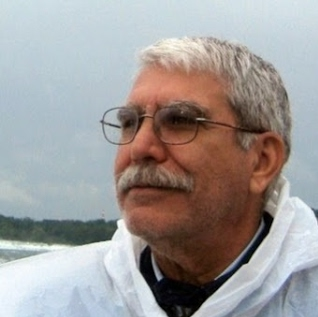
\includegraphics[width=0.70\textwidth]{Figures/DocBouzas} 
%\decoRule
\caption[Foto Sorpresa]{En esta figura se muestra al mejor doc del mundo}
\label{Figura}
\end{figure}



\begin{center}
Tercero, las citas y referencias.\\
\end{center}

En general, puedes referir cualquier elemento que hayas insertado en el texto y al cual le hayas asignado una "label" (ver código para que esto tenga sentido). Es decir, aplica para imágenes, tablas y ecuaciones...\\

Por ejemplo! Podemos referirnos aquí a nuestra bella fotografía presentada con anterioridad en la Figura~\ref{Figura}\\

En cuanto a las referencias bibliográficas, este template está hecho para que las citas aparezcan en el trabajo en paréntesis, agregando automáticamente (en formato APA) todos aquellos trabajos que hayas referido durante tu redacción. (En otras palabras, lo que aparezca en la bibliografía es un reflejo estricto del contenido de tu trabajo... No se vale inflar las Referencias con trabajos que no vas a usar) \parencite{Articulo, Libro, Capitulo}\\
